\documentclass{article}
\usepackage{amsfonts, amsmath, amssymb, amsthm} % Math notations imported
\usepackage{enumitem}
\usepackage{graphicx}
\usepackage{setspace}
\usepackage{indentfirst}
\usepackage[margin=1in]{geometry}
\graphicspath{{./images/}} % Path to images

% \begin{figure}[htb!]
%      \centering
%      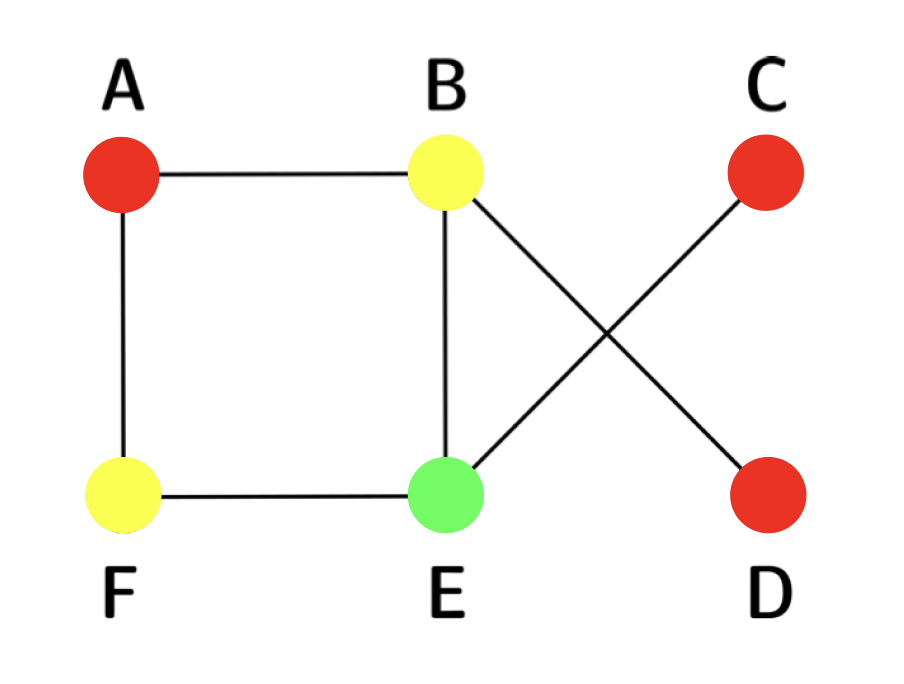
\includegraphics[scale=0.5]{coloring.png}
%      \caption{Coloring of the graph.}
% \end{figure}

\newtheorem{thm}{Theorem}
\newtheorem{proposition}[thm]{Proposition}
\newtheorem{cor}[thm]{Corollary}

% title information
\title{Math 110 HW2}
\author{Neo Lee}
\date{09/09/2023}

\setstretch{1.15}
% main content
\begin{document} 

% placing title information; comment out if using fancyhdr
\maketitle 

\subsection*{Problem 1.}
Suppose $U:=\{(x,x,3x):x\in\mathbb{R}\}$ and $W:=\{(x,-x,-3x):x\in\mathbb{R}\}$. 
\begin{enumerate}[label=(\alph*)]
    \item \begin{proposition}
        $U$ and $W$ are subspaces of $\mathbb{R}^3$.
    \end{proposition}
    \item Describe $U+W$ using symbols.
    \item Describe $U+ W$ without symbols.
\end{enumerate}

\subsection*{Problem 2.}
Suppose $\mathbb{F}=\mathbb{R}$ or $\mathbb{F} = \mathbb{C}$ and let 
$$U = \{(x,y,x+y,-y,-x)\in\mathbb{F}^5:x,y\in\mathbb{F}\}.$$
Find three subspaces $W_1, W_2, W_3$ of $\mathbb{F}^5$, none of which equals \{0\}, such that 
$\mathbb{F}^5=U\oplus W_1\oplus W_2\oplus W_3$.

\subsection*{Problem 3.}
\begin{proposition}
    Let $V$ be a vector space over $\mathbb{F}$. Suppose that $1+1\neq 0$ in $\mathbb{F}$ and the 
    list $v_1,v_2,v_3,v_4$ is linearly independent in $V$. Then the list $v_1-v_2,v_1+v_2,v_3-v_2
    ,v_4-v_1$ is also linearly independent in $\mathbb{V}$.
\end{proposition}

\subsection*{Problem 4.}
Does the statement of Problem 3 still hold if we replace "linearly independent" by "a basis"?

\subsection*{Problem 5.}
\begin{proposition}
    The space $\mathbb{R}^{[0,1]}$ is infinite-dimensional.
\end{proposition}

\end{document}
